%%%%%%%%%%%%%%%%%%%%%%%%%%%%%%%%%%%%%%%%%%%%%%%%%%%%%%%
% % Lines starting with % are comments, which are ignored.
% % This is a handy way of indicating the date and version of
% % your document, to wit:
% %
% % LaTeX sample file
% % Modified March, 2002
% %
%%%%%%%%%%%%%%%%%%%%%%%%%%%%%%%%%%%%%%%%%%%%%%%%%%%%%%%
\DocumentMetadata{
  % PDF standards: ONE key whose value is a comma-separated list --
  % UA-2 (accessibility) plus A-4f (archival; the archival companion of
  % UA-2). Do NOT use separate pdfstandard=... keys: with ordinary
  % key-value parsing only the last one takes effect.
  pdfstandard={UA-2,A-4f},
  lang=en-US,
  tagging=on,
  tagging-setup={
    math/setup=mathml-SE
  }
}

\documentclass[12pt]{exam}
% worksheet-macros.tex -- shared package setup for worksheet-template.tex.
%
% NOTE ON PATHS: every template in this repository is stored one level up
% from where it is compiled (see README.md). All relative \input paths
% below are resolved against the folder the document is compiled in,
% which sits one directory above this file.

% --- Math ------------------------------------------------------------
% amsmath: equation environments and numbering
% amsfonts: \mathbb etc.  |  mathrsfs: \mathfrak  |  stmaryrd: extra symbols
\usepackage{amsmath}
\usepackage{amsfonts}
\usepackage{mathrsfs}
\usepackage{stmaryrd}

% --- Layout and glyphs ------------------------------------------------
% float: [H] float placement (stop floats where you put them)
% fontspec: Unicode/OpenType fonts (compile with XeLaTeX or LuaLaTeX)
% emoji: emoji glyphs in the text
\usepackage{float}
\usepackage{fontspec}
\usepackage{emoji}

% --- Typography --------------------------------------------------------
% Atkinson Hyperlegible as the document-wide sans serif (sfdefault):
% a high-legibility face that is easier to read for students with
% dyslexia or low vision.
\usepackage[sfdefault]{atkinson}

% --- Colors -------------------------------------------------------------
% dvipsnames: extended named color palette (the Accessible* colors in
%   lecture-macros.tex are built on it);
% table: \rowcolors / \cellcolor for shading worksheet tables.
% NOTE: xcolor may only be loaded ONCE per document -- a second
% \usepackage{xcolor} with different options is a fatal "Option clash"
% error, so ALL of its options are listed here.
\usepackage[dvipsnames,table]{xcolor}

% --- Multimedia ---------------------------------------------------------
% animate: embeds audio/video (and legacy Flash) media in the worksheet.
\usepackage{animate}

% --- Bibliography --------------------------------------------------------
% biblatex (biber backend): citations and a reference list for worksheets.
\usepackage[
  backend=biber,
  style=alphabetic,
  url=true,
  doi=true,
  isbn=true,
  backref=true
]{biblatex}

% --- Links ---------------------------------------------------------------
% hyperref makes every \ref/citation/URL clickable in the PDF.
% Link colors must satisfy WCAG 1.4.3 (>= 4.5:1 contrast on white):
%   blue = 8.6:1, green!40!black = 7.2:1.
% (The old cyan/magenta values measured 1.25:1 / 3.1:1 and failed.)
\usepackage{hyperref}
\hypersetup{
  colorlinks=true,
  linkcolor=blue,
  filecolor=blue,
  urlcolor=green!40!black,
}

% --- Shared course macros ------------------------------------------------
% Root macros.tex: math shorthands used across all course documents
% (\RR, \NN, \ZZ, \QQ, \grad, \curl, \tr, \der, \pder, ...).
\newcommand{\RR}{\mathbb{R}}
\newcommand{\NN}{\mathbb{N}}
\newcommand{\ZZ}{\mathbb{Z}}
\newcommand{\QQ}{\mathbb{Q}}
\newcommand{\vv}{\vec{v}}
\newcommand{\ww}{\vec{w}}
\newcommand{\xx}{\vec{x}}
\newcommand{\yy}{\vec{y}}
\newcommand{\zz}{\vec{z}}
\newcommand{\uu}{\vec{u}}
\newcommand{\basis}[1]{\vec{e_{#1}}}
\newcommand{\id}{\mathrm{id}}
\newcommand{\CC}{\mathbb{C}}
\renewcommand{\div}{\operatorname{div}}
\newcommand{\grad}{\operatorname{grad}}
\newcommand{\curl}{\operatorname{curl}}
\newcommand{\tr}{\operatorname{tr}}
\newcommand{\der}[2]{\dfrac{d #1}{d #2}}
\newcommand{\pder}[3][]{\dfrac{\partial^{#1} #2}{\partial #3}}


% % Title and author(s)
%%%%%%%%%%%%%%%%%%%%%%%%%%%%%%%%%%%%%%%%%%%%%%%%%%%%%%%
\title{Worksheet 12 - Inverse and Implicit Differentiation}
\author{MATH 1271}
\date{10/20/2026}
%%%%%%%%%%%%%%%%%%%%%%%%%%%%%%%%%%%%%%%%%%%%%%%%%%%%%%%
% %
% % The next command allows your in import encapsulated
% % postscript files, .epsf or .eps files, which
% % contain vector graphic image data.
% %
%%%%%%%%%%%%%%%%%%%%%%%%%%%%%%%%%%%%%%%%%%%%%%%%%%%%%%%
% %   The first thanks indicates your affiliation
% %
% %  Just the name here.
% %
% % Your mailing address goes at the end.
% %
% % \thanks is also how you indicate grant support
% %
%%%%%%%%%%%%%%%%%%%%%%%%%%%%%%%%%%%%%%%%%%%%%%%%%%%%%%%

%%%%%%%%%%%%%%%%%%%%%%%%%%%%%%%%%%%%%%%%%%%%%%%%%%%%%%%
% $ The next command ensures the margins are 1 inch on
% % all sides.
% %
%%%%%%%%%%%%%%%%%%%%%%%%%%%%%%%%%%%%%%%%%%%%%%%%%%%%%%%
\begin{document}
\newpage
\maketitle

\begin{enumerate}

  \item For the following functions, determine their derivatives by recognizing them as inverse functions and applying inverse function rule.

    \begin{enumerate}
      \item $f(x) = \sqrt[n]{x}$.

        \vfill

      \item $g(x) = \log_c(x)$.
        \vfill

      \item $h(x) = \operatorname{arccot}(x)$.
        \vfill
    \end{enumerate}

    \newpage

  \item For the following parts, let
    \begin{equation*}
      f(x) = x^4 - 2x^3 + 3x^2 - 2x + 1.
    \end{equation*}

    \begin{enumerate}
      \item Compute $f(1)$.
        \vfill

      \item Use the previous part to compute $f^{-1}(1)$.
        \vfill

      \item What is the derivative of $f^{-1}(x)$ at $x = 1$?
        \vfill

      \item For which values of $x$ is the line tangent to $y = f^{-1}(x)$
        at $(x, f^{-1}(x))$ horizontal? For which values of $x$ is it vertical?
        \vfill
    \end{enumerate}

  \newpage

\item For each of the following equations, use implicit differentiation to find $\frac{dy}{dx}$, and determine the value of the derivative at the given point.

\begin{enumerate}

\item $x^3-y^3=6xy$; $(-3,3)$

\vfill

\item $\sin(y)+y=x^3+x$; $(0,0)$

\vfill

\item $e^{x/y}=x-y$; $(0, -1)$

\vfill

\end{enumerate}



\newpage

\item Consider the curve defined by the equation $y(y^2-1)(y-2)=x(x-1)(x-2)$, whose graph is pictured below:

\begin{center}
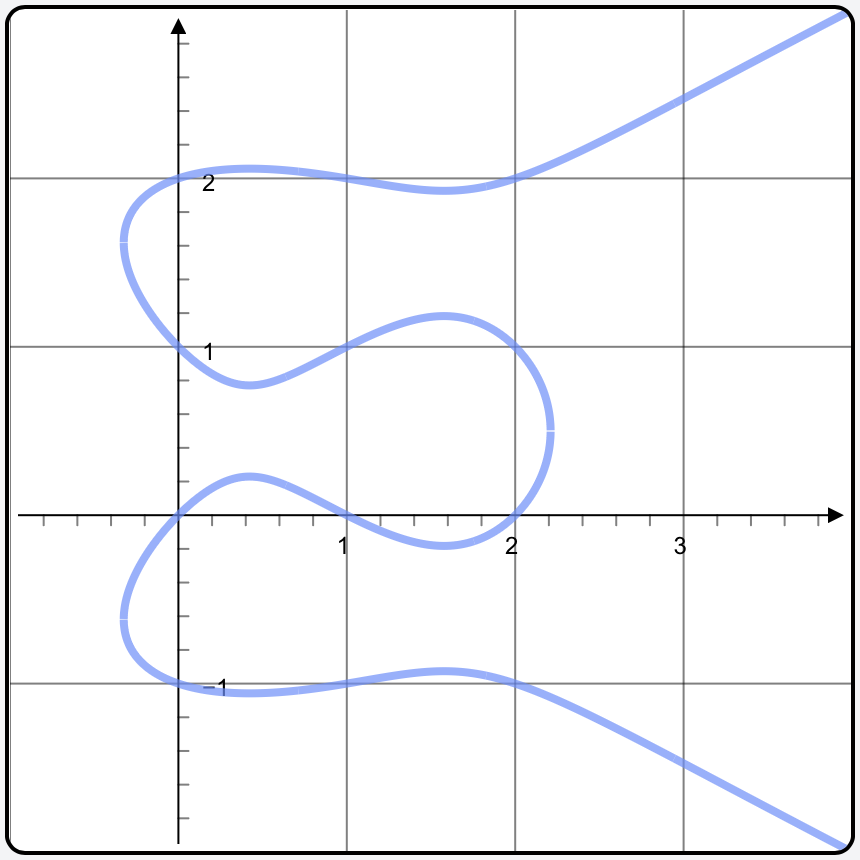
\includegraphics[scale=0.5]{wkst13img-f25}
\end{center}

Through implicit differentiation, it can be shown that
$$\frac{dy}{dx}=\frac{(x-1)(x-2)+x(x-2)+x(x-1)}{(y^2-1)(y-2)+2y^2(y-2)+y(y^2-1)}$$

Use this fact to answer each of the following questions with $3$ decimal points of accuracy.

\begin{enumerate} 

\item Determine all values of $x$ at which the tangent line to the curve is horizontal.

\emph{Note: You may--and should!--use technology, such as \href{http://www.wolframalpha.com}{wolframalpha.com}, to find the needed zeros of the relevant polynomial function. For example, to have WolframAlpha solve the equation $x^2-3x+1=0$ for you, type "Solve $x^2-3x+1=0$" into the search box. It will output the answers $x=\frac{1}{2}(3-\sqrt{5})$ and $x=\frac{1}{2}(3+\sqrt{5})$.}

\vfill

\item Determine all points $(x,y)$ at which the tangent line to the curve is horizontal.

\vfill

\newpage

\item Determine all points $(x,y)$ at which the tangent line to the curve is vertical.

\vfill

\item Find the equation (in slope-intercept form) of the tangent line to the curve at one of the points where $x=1$.

\vspace{3.5in}

\end{enumerate}


\end{enumerate}

% Most people don't use these, so they are "commented out"
% by starting the lines with a "%"
%\begin{keywords}
%   \LaTeX, typesetting
%\end{keywords}

%\begin{AMS}
%   50C60, 18C25
%\end{AMS}

%%%%%%%%%%%%%%%%%%%%%%
% % Here is the start of the Text
%%%%%%%%%%%%%%%%%%%%%%
\end{document}
